% \section{Appendix Section}
% \label{sec:appendix_section}
\maketitlesupplementary
\setcounter{figure}{5}
\setcounter{table}{6} 

This supplementary document complements the main manuscript by providing expanded quantitative analyses and qualitative visualizations of PatchAlign3D. First, Section A presents comprehensive ablation studies that validate our architectural design choices, specifically evaluating the impact of different dense 2D visual encoders, text encoders, and Stage 2 freezing strategies. We also provide additional qualitative comparisons in Section B, illustrating the robustness of our patch-level alignment in both text-to-feature and anchor-based scenarios. Finally, we detail our experimental framework for zero-shot and few-shot keypoint detection in Section C, demonstrating the method's fine-grained capabilities and potential for additional applications.

\section{Additional Ablations}


\begin{table}[t]
    \centering
    \begin{tabular}{lcc}
        \toprule
        2D encoder & mIoU & cIoU \\
        \midrule
        DINOv1~\cite{caron2021emerging} & 51.82 & 54.39 \\
        DINOv3~\cite{simeoni2025dinov3} & 46.52 & 42.76 \\
        OpenCLIP ViT-bigG-14 ~\cite{radford2021learning}& 49.32 & 52.96 \\
        DINOv2~\cite{oquab2023dinov2}(ours) & \textbf{56.90} & \textbf{53.10} \\
        \bottomrule
    \end{tabular}
    \caption{\textbf{Ablation on the 2D encoder used during Stage 1.}
    We evaluate several dense visual encoders for multi-view 2D feature distillation.
    All models produce competitive results, but dense-trained ViTs~\cite{dosovitskiy2020image} such as
    DINOv1 and DINOv2 perform best, supporting our choice of DINOv2.}
    \label{tab:2d_encoder_ablation}
\end{table}

\paragraph{Ablation on the 2D visual encoder.}
\cref{tab:2d_encoder_ablation} shows that PatchAlign3D is compatible with any
visual encoder that produces dense spatial features. ViT-based~\cite{dosovitskiy2020image} models such as
DINOv1~\cite{caron2021emerging}, CLIP~\cite{radford2021learning}, and DINOv2~\cite{oquab2023dinov2} all yield strong results, demonstrating that Stage 1
distillation does not depend on a specific visual backbone. Dense representation
learning appears particularly important: DINOv1~\cite{caron2021emerging} and DINOv2~\cite{oquab2023dinov2}, both trained with
dense objectives, outperform CLIP. Surprisingly, DINOv3~\cite{simeoni2025dinov3} severely underperforms, possibly
because its features are optimized for more fine-grained objectives and are
less suitable for shape segmentation, showing that the passage from DINOv2 to DINOv3 is not necessarily beneficial for all downstream tasks. These results justify our
use of DINOv2~\cite{oquab2023dinov2} for the main experiments.



\begin{table}[t]
    \centering
    \begin{tabular}{lcc}
        \toprule
        Text encoder & mIoU & cIoU \\
        \midrule
        SigLIP~\cite{zhai2023sigmoid} & 46.44 & 40.51 \\
        OpenCLIP ViT-bigG-14~\cite{radford2021learning} (ours) & \textbf{56.90} & \textbf{53.10} \\
        Gemma-2-9B-it~\cite{team2024gemma}& 54.83 & 50.98 \\
        \bottomrule
    \end{tabular}
    \caption{\textbf{Ablation on the text encoder.}
    All text encoders yield substantial improvements over prior baselines.
    CLIP ViT-bigG~\cite{radford2021learning} remains the strongest, but even purely textual encoders such as
    Gemma-2-9B-it~\cite{team2024gemma} perform surprisingly well, indicating that Stage 2 does not strictly
    require a vision–language pre-trained text tower.}
    \label{tab:text_encoder_ablation}
\end{table}

\paragraph{Ablation on the text encoder.}
As shown in \cref{tab:text_encoder_ablation}, PatchAlign3D performs well with
a range of text encoders. The CLIP ViT-bigG~\cite{radford2021learning} model achieves the best results,
likely due to its large-scale multimodal training. However, the performance of
Gemma-2-9B-it~\cite{team2024gemma}, despite being trained purely on text, is notable and indicates that Stage 2 learning does not rely on a
visually-grounded text tower. This highlights the robustness of our
multi-positive patch-level alignment mechanism.



\begin{table}[t]
    \centering
    \begin{tabular}{lcc}
        \toprule
        Freezing strategy & mIoU & cIoU \\
        \midrule
        Freeze last block (ours) & \textbf{56.90} & \textbf{53.10} \\
        Freeze last two blocks & 55.70 & 50.93 \\
        Freeze last three blocks & 55.24 & 49.62 \\
        Full encoder frozen & 53.95 & 50.10 \\
        Full fine-tuning & 49.40 & 48.75 \\
        \bottomrule
    \end{tabular}
    \caption{\textbf{Ablation on the freezing strategy during Stage 2.}
    We freeze most of the encoder to preserve Stage 1 visual knowledge and
    avoid destructive interference with the text-alignment objective. Best
    results are obtained by unfreezing only the projection head and the final
    transformer block.}
    \label{tab:freezing_ablation}
\end{table}

\paragraph{Ablation on the freezing strategy.}
Stage 1 provides high-quality geometric and semantic priors, and Stage 2 must
align them to text without overriding these learned representations.  
\cref{tab:freezing_ablation} shows that fully fine-tuning the encoder harms
performance, indicating that the text objective alone is not sufficient to
preserve Stage 1 knowledge. Conversely, freezing the entire encoder limits the
ability to adapt to the language space.  
The best trade-off is obtained by freezing all but the last transformer block
and the projection head, which allows for gentle adaptation while preserving
most Stage 1 features. This strategy is used in PatchAlign3D.


\section{Additional Qualitative Comparisons}

\begin{figure}[t]
    \centering
    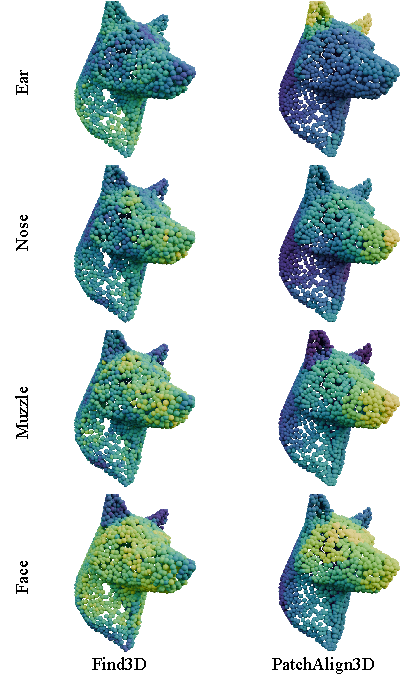
\includegraphics[width=\columnwidth]{figs/supplementary/qualitative_text.pdf}
    \caption{\textbf{Text-to-feature similarity visualization.}
    We compare PatchAlign3D to Find3D by visualizing similarities between a
    textual query (e.g., \emph{``ear''}, \emph{``nose''}) and the dense features
    on a validation point cloud. Yellow indicates higher similarity.
    PatchAlign3D produces sharper and more localized responses, while Find3D
    often shows diffuse signals with weaker semantic localization.}
    \label{fig:qualitative_text}
\end{figure}

\paragraph{Text-to-feature similarity.}
Figure~\ref{fig:qualitative_text} highlights the difference between our
patch-level alignment and Find3D's~\cite{ma2025find} point-wise contrastive learning. Find3D's
responses are often noisy and lack spatial precision, whereas PatchAlign3D
produces clean, well-localized activations that align closely with the queried
part. Related queries (e.g., \emph{``nose''} vs. \emph{``muzzle''}) activate
similar regions, demonstrating semantic consistency in the learned feature
space.


\begin{figure}[t]
    \centering
    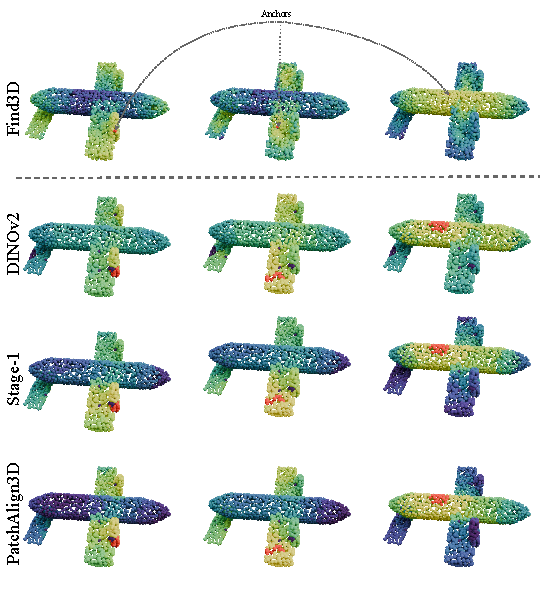
\includegraphics[width=\columnwidth]{figs/supplementary/qualitative_anchor.pdf}
    \caption{\textbf{Anchor-based feature similarity.}
    For a selected anchor point or patch on a shape (e.g., wing, body, motor),
    we visualize the similarity of all other points/patches to the anchor.
    PatchAlign3D shows stronger geometric coherence than DINOv2, Stage 1, and
    Find3D.}
    \label{fig:qualitative_anchor}
\end{figure}

\paragraph{Anchor-based feature similarity.}
Figure~\ref{fig:qualitative_anchor} provides deeper insight into the structure
of the learned representations. DINOv2~\cite{oquab2023dinov2} features exhibit limited contrast and
lack clear part boundaries. Stage 1 improves geometric coherence but may
preserve symmetries or artifacts from multi-view lifting. Find3D~\cite{ma2025find} captures part
structure but with weaker separation between fine-grained regions.
PatchAlign3D produces the cleanest and most discriminative part clusters,
demonstrating that Stage 2 refines Stage 1 features while preserving geometric
priors.

\section{Zero-shot and Few-shot Keypoint Detection}

In this section, we introduce a zero-shot approach for keypoint detection on 3D shapes. Compared to semantic segmentation, reasoning at the point level on visual data is challenging because it requires precise localization capabilities, which can be problematic even for advanced models like GPT-4o~\cite{achiam2023gpt} and PaliGemma 2~\cite{steiner2024paligemma}.

Traditionally, 3D keypoint detection relies heavily on annotated 3D datasets and extensive supervised training, which limits its scalability and its applicability to new categories or domains. In contrast, the zero-shot method takes advantage of the rich knowledge embedded within language models. Specifically, we show that part-level annotations used to train 3D encoders can be employed to detect salient keypoints on 3D models without requiring any ground truth labels or supervision.

We evaluate our method using the KeypointNet dataset, which provides dense annotations and text prompts for keypoints. Our evaluation strategy and baselines are based on the method described by 
\citet{gong2025zerokey}. This evaluation computes the Intersection over Union (IoU) between predicted keypoints and ground-truth keypoints from the KeypointNet~\cite{you2020keypointnet} dataset, using different distance thresholds. A match is counted when the geodesic distance between a ground-truth keypoint and a predicted keypoint is less than the specified threshold.

\begin{table*}[t]
\centering
\begin{tabular}{lccccccccccc}
\toprule
\textbf{Method} & \textbf{0.001} & \textbf{0.01} & \textbf{0.02} & \textbf{0.03} & \textbf{0.04} & \textbf{0.05} & \textbf{0.06} & \textbf{0.07} & \textbf{0.08} & \textbf{0.09} & \textbf{0.10} \\
\midrule
HARRIS-3D~\cite{sipiran2011harris} & 0.15 & 0.76 & 2.19 & 3.96 & 6.16 & 8.88 & 11.91 & 15.13 & 18.63 & 22.10 & 25.69 \\
SIFT-3D~\cite{rister2017volumetric} & 0.29 & 1.05 & 2.62 & 4.83 & 6.95 & 9.42 & 12.38 & 15.65 & 19.39 & 22.71 & 26.15 \\
ISS~\cite{zhong2009intrinsic} & 0.32 & 1.19 & 2.79 & 4.76 & 6.93 & 9.40 & 12.04 & 15.10 & 18.32 & 22.08 & 25.87 \\
USIP~\cite{li2019usip} & 0.83 & 1.70 & 3.25 & 5.24 & 8.07 & 11.15 & 15.98 & 20.56 & 25.36 & 30.16 & 34.77 \\
D3FEAT~\cite{bai2020d3feat} & 2.36 & 3.86 & 7.82 & 12.77 & 18.53 & 25.02 & 31.14 & 36.65 & 41.74 & 46.33 & 50.52 \\
UKPGAN~\cite{you2022ukpgan} & 3.95 & 6.54 & 12.77 & 18.22 & 26.45 & 35.32 & 40.28 & 34.42 & 42.65 & 46.05 & 46.49 \\
FSKD~\cite{attaiki2022ncp} & 7.00 & 7.94 & 11.17 & 17.67 & 23.99 & 31.14 & 38.14 & 43.97 & 49.32 & 53.87 & 57.05 \\
B2-3D~\cite{wimmer2024back} & 6.20 & 11.87 & 19.63 & 27.65 & 31.14 & 34.64 & 38.86 & 41.95 & 44.77 & 46.69 & 49.25 \\
ULIP-2~\cite{xue2023ulip} & 2.00 & 3.85 & 7.09 & 9.31 & 11.22 & 13.11 & 15.23 & 17.57 & 19.95 & 22.34 & 24.88 \\
\specialrule{0.5pt}{1pt}{1pt} % Light separator above our method
\rowcolor{blue!10}
\begin{tabular}{@{}l@{}} PatchAlign3D \\ - Few Shot (Ours) \end{tabular}
& \textbf{7.80} & \textbf{12.16} & \textbf{21.63} & \textbf{30.54} & \textbf{37.48} & \textbf{43.61} & \textbf{48.96} & \textbf{53.51} & \textbf{57.46} & \textbf{60.97} & \textbf{64.07} \\
\midrule
PaliGemma 2~\cite{steiner2024paligemma} & 0.00 & 0.34 & 1.03 & 2.98 & 4.93 & 7.00 & 6.62 & 8.17 & 8.92 & 11.49 & 11.56 \\
RedCircle~\cite{shtedritski2023does} & 0.21 & 0.34 & 0.64 & 1.16 & 1.90 & 3.04 & 4.81 & 7.55 & 11.06 & 14.92 & 18.50 \\
GPT-4o~\cite{achiam2023gpt} & 0.28 & 0.38 & 1.04 & 2.11 & 4.79 & 6.58 & 8.48 & 10.09 & 14.03 & 17.03 & 17.85 \\
CLIP-DINoiser~\cite{wysoczanska2024clip} & 0.73 & 1.41 & 3.00 & 4.94 & 7.31 & 9.81 & 12.66 & 15.52 & 18.52 & 21.76 & 25.56 \\
\specialrule{0.5pt}{1pt}{1pt} % Light separator above our method
\rowcolor{green!12}
\begin{tabular}{@{}l@{}} PatchAlign3D \\ - Zero Shot (Ours) \end{tabular}
& \textbf{2.21} & \textbf{3.94} & \textbf{9.48} & \textbf{16.13} & \textbf{19.88} & \textbf{22.04} & \textbf{23.32} & \textbf{25.23} & \textbf{27.85} & \textbf{31.44} & \textbf{32.88} \\
\bottomrule
\end{tabular}
\caption{Comparison of IoU between the predicted and ground-truth keypoints from KeypointNet using different methods across various geodesic distance thresholds. The \textbf{\colorbox{blue!10}{blue}} text indicates the best few-shot methods, while the \textbf{\colorbox{green!10}{green}} text highlights the best zero-shot methods.}
\label{tab:comparison_suppl}
\end{table*}

\begin{figure}[t]
    \vspace{-2em}
    \centering
    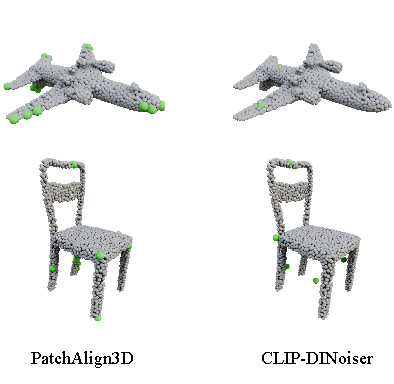
\includegraphics[width=\columnwidth]{figs/supplementary/keypoint.pdf}
    \caption{\textbf{Visualization of keypoints detected in zero-shot keypoint detection.} In these experiments, the input to our method is a point cloud containing 2048 points. The detected keypoints given a text prompt are highlighted as larger green dots.}
    \label{fig:qualitative_kp}
\end{figure}

Among all the baselines, both RedCircle~\cite{shtedritski2023does} and CLIP-DINOiser~\cite{wysoczanska2024clip} utilize text alignment from CLIP, allowing for the querying of keypoints using text in a zero-shot setting. However, both methods are multiview-based and do not incorporate explicit 3D modeling. Our approach also leverages CLIP for feature alignment with text, but it benefits from a 3D point encoder. This makes RedCircle and CLIP-DINOiser ideal baselines for comparison with our method.

Our evaluation of KeypointNet~\cite{you2020keypointnet} demonstrates (refer to Fig. \ref{fig:qualitative_kp} and Tab. \ref{tab:comparison_suppl}) that our text-aligned local feature significantly outperforms other baselines, including RedCircle, CLIP-DINOiser, and even GPT-4o, across all distance thresholds. Additionally, in few-shot settings where text alignment is not required, our patch-adopted feature significantly surpasses the globally adopted ULIP-2~\cite{xue2023ulip} features and the multi-view aggregated features from B2-3D.

This provides strong evidence that our language-aligned local features are not only more semantically meaningful but also serve as better geometry descriptors compared to globally supervised features. Furthermore, our method achieves IoU levels comparable to those of supervised methods specifically designed for this dataset, such as B2-3D~\cite{wimmer2024back} and FSKD~\cite{attaiki2022ncp}. These results emphasize that our feature improved point-level understanding of both text semantics and geometry through fine-grained patch alignment.

